% =====================================================================
%  Subsistemas añadidos al modelo Drone.mo
%  Documento autónomo: cada sección de ./secciones puede copiarse o
%  incluirse con \input{} en el informe principal (Modelado_Trabajo).
% =====================================================================
\documentclass[11pt,a4paper]{article}

\usepackage[utf8]{inputenc}
\usepackage[T1]{fontenc}
% Español si está instalado (Overleaf / texlive-lang-spanish); si no, inglés
\IfFileExists{spanish.ldf}
  {\usepackage[spanish,es-noshorthands,es-tabla]{babel}}
  {\usepackage[english]{babel}}
\usepackage{amsmath,amssymb}
\usepackage{geometry}
\geometry{margin=2.5cm}
\usepackage{booktabs}
% siunitx si está instalado; si no, sustituto mínimo de \SI y \si
\IfFileExists{siunitx.sty}
  {\usepackage{siunitx}\sisetup{output-decimal-marker={,}}}
  {% Sustituto mínimo de siunitx (solo si el paquete no está instalado)
\providecommand{\ohm}{\Omega}
\newcommand{\si}[1]{\ensuremath{\mathrm{#1}}}
\newcommand{\SI}[2]{\ensuremath{#1\,\mathrm{#2}}}
}
\usepackage{listings}
\usepackage{xcolor}
\usepackage{tikz}
\usetikzlibrary{arrows.meta,positioning}
\usepackage{hyperref}

% Definición del lenguaje Modelica para el paquete listings
\lstdefinelanguage{Modelica}{
  morekeywords={model,block,end,equation,initial,parameter,input,output,
    import,within,extends,connect,annotation,if,then,else,elseif,for,in,
    loop,protected,public,der,inner,outer,each,final,and,or,not,true,false,
    Real,Boolean,Integer,sum,min,max,abs,sqrt,zeros,time},
  sensitive=true,
  morecomment=[l]{//},
  morecomment=[s]{/*}{*/},
  morestring=[b]",
}
\lstset{
  language=Modelica,
  basicstyle=\ttfamily\footnotesize,
  keywordstyle=\color{blue!70!black}\bfseries,
  commentstyle=\color{green!45!black}\itshape,
  stringstyle=\color{red!60!black},
  numbers=left,
  numberstyle=\tiny\color{gray},
  frame=single,
  breaklines=true,
  showstringspaces=false,
  columns=fullflexible,
  literate={á}{{\'a}}1 {é}{{\'e}}1 {í}{{\'i}}1 {ó}{{\'o}}1 {ú}{{\'u}}1 {ñ}{{\~n}}1,
}


\title{Subsistemas eléctrico, de propulsión y de perturbaciones\\
       \large Ampliación del modelo \texttt{ModeloDrone.Drone}}
\author{Modelado y Simulación de Sistemas -- Grupo I}
\date{}

\begin{document}
\maketitle

\section{Elementos añadidos al modelo}
\label{sec:resumen}

El modelo \texttt{Drone.mo} implementaba la dinámica del cuerpo rígido, la matriz de
asignación y su inversa, y el lazo de control en cascada
(posición $\rightarrow$ velocidad $\rightarrow$ actitud). En él, las velocidades de los
rotores calculadas por $A^{-1}$ se aplicaban directamente a la matriz de asignación,
como si los motores fuesen ideales.

Para cumplir con el alcance definido en el \emph{Informe~1} y en el documento de
\emph{Modelado y simulación de cuadricóptero} se han añadido los siguientes
subsistemas, cada uno como un componente Modelica independiente:

\begin{itemize}
  \item \textbf{Motores} (\texttt{SubSistemas.ModeloMotor}): modelo equivalente de
        motor de corriente continua con su dinámica eléctrica y mecánica y la carga
        de la hélice (Informe~1, ecs.~3--8).
  \item \textbf{Controlador de velocidad / ESC} (\texttt{SubSistemas.ESC}): convierte
        las velocidades de referencia $\omega_i^{*}$ en las tensiones $V_i$, que son
        las entradas físicas del sistema (Modelado, ec.~32), con
        $0 \le V_i \le V_{bat}$.
  \item \textbf{Batería} (\texttt{SubSistemas.Bateria}): reserva de energía con
        $\dot E = -P$ (Informe~1, ec.~9).
  \item \textbf{Carga transportada}: $m_{total} = m_d + m_c$ (Informe~1, ec.~1;
        Modelado, ec.~41).
  \item \textbf{Perturbaciones} (\texttt{SubSistemas.Perturbaciones}): resistencia
        aerodinámica $\mathbf{F}_d$ y viento $\mathbf{F}_{wind}$ (Modelado, ecs.~8
        y~40).
\end{itemize}

Con ello, la cadena de causa y efecto del sistema queda completa:
\begin{equation}
  \text{Batería} \rightarrow V_i \rightarrow i_i \rightarrow \omega_i
  \rightarrow F_i,\,Q_i \rightarrow \mathbf{F},\,\boldsymbol{\tau}
  \rightarrow \text{Movimiento}
\end{equation}

\paragraph{Sistema de referencia.} No se ha modificado el sistema de referencia del
modelo. El sistema inercial (\texttt{world}) mantiene la gravedad en $-z$
($\mathbf{n} = [0\;0\;-1]^T$, eje $z$ vertical hacia arriba). El empuje sigue
aplicándose sobre el eje $z$ del cuerpo (\texttt{forceAndTorque} resuelto en
\texttt{frame\_b}), y los sensores de posición y velocidad siguen expresados en el
sistema inercial. Las nuevas fuerzas de perturbación se definen directamente en el
sistema inercial.

\section{Subsistema de los motores}
\label{sec:motor}

Cada motor sin escobillas, junto con su controlador electrónico, se representa mediante
un modelo equivalente de motor de corriente continua. La tensión $V_i$ es la tensión
equivalente aplicada al motor $i$, con $i = 1,\dots,4$.

\subsection{Modelo eléctrico}
\begin{equation}
  V_i = R\, i_i + L \frac{d i_i}{dt} + k_e\, \omega_i
  \qquad\Longrightarrow\qquad
  \frac{d i_i}{dt} = \frac{1}{L}\left(V_i - R\, i_i - k_e\, \omega_i\right)
  \label{eq:motor_elec}
\end{equation}

\subsection{Modelo mecánico}
El par electromagnético es $\tau_{m,i} = k_t\, i_i$. La hélice ejerce un par resistente
proporcional al cuadrado de la velocidad, que es el mismo par de reacción $Q_i$ que
aparece en la matriz de asignación:
\begin{equation}
  \tau_{p,i} = Q_i = k_m\, \omega_i^2
  \label{eq:motor_tau_p}
\end{equation}
\begin{equation}
  J_m \frac{d\omega_i}{dt} = k_t\, i_i - k_m\, \omega_i^2 - b_m\, \omega_i
  \label{eq:motor_mec}
\end{equation}

En la implementación se escribe $k_m\,\omega_i\,|\omega_i|$, que es idéntico a
$k_m\,\omega_i^2$ para $\omega_i \ge 0$ y mantiene el signo correcto del par si el
rotor llegase a girar en sentido contrario.

\subsection{Empuje generado}
La velocidad $\omega_i$ que sale de cada motor es la entrada de la matriz de asignación
(Modelado, ec.~29), que calcula
\begin{equation}
  F_i = k_f\, \omega_i^2, \qquad F_z = \sum_{i=1}^{4} F_i ,
\end{equation}
donde $k_f$ es el coeficiente de empuje ($k_T$ en el Informe~1).

\subsection{Potencia eléctrica}
\begin{equation}
  P_{el,i} = V_i\, i_i
\end{equation}

\subsection{Condición inicial}
Por defecto (\texttt{steadyStateInit = true}) la simulación arranca con los motores en
régimen estacionario, $\dot i_i = 0$ y $\dot\omega_i = 0$. Como valor inicial de
iteración se usa la velocidad de vuelo estacionario
\begin{equation}
  \omega_h = \sqrt{\frac{m_{total}\, g}{4 k_f}} .
\end{equation}

\subsection{Estados}
Cada motor aporta dos estados, $i_i$ y $\omega_i$. Los cuatro motores aportan
\begin{equation}
  \mathbf{x}_m = \begin{bmatrix} i_1 & i_2 & i_3 & i_4 & \omega_1 & \omega_2 & \omega_3 & \omega_4 \end{bmatrix}^T ,
\end{equation}
que, junto con los 12 estados del cuerpo rígido $\mathbf{x}_b$ (Modelado, ec.~20),
dan los 20 estados físicos de $\mathbf{x} = [\mathbf{x}_b^T\;\mathbf{x}_m^T]^T$
(Modelado, ec.~31).

\section{Controlador de velocidad de los motores (ESC equivalente)}
\label{sec:esc}

La matriz de asignación inversa (Modelado, ec.~30) proporciona las velocidades
deseadas $\omega_i^{*}$, saturadas a $0 \le \omega_i^{*} \le \omega_{max}$
(Modelado, ec.~42). Sin embargo, las entradas físicas del sistema son las tensiones
de los motores, $\mathbf{u} = [V_1\;V_2\;V_3\;V_4]^T$ (Modelado, ec.~32). El bloque
ESC cierra un lazo PI de velocidad por motor con un término de prealimentación
basado en el modelo del motor.

\subsection{Prealimentación}
Imponiendo $\dot i_i = 0$ y $\dot\omega_i = 0$ en \eqref{eq:motor_elec} y
\eqref{eq:motor_mec} con $\omega_i = \omega_i^{*}$ se obtiene la tensión de régimen
permanente:
\begin{equation}
  V_{ff,i} = k_e\, \omega_i^{*} + \frac{R}{k_t}\left(k_m\, {\omega_i^{*}}^2 + b_m\, \omega_i^{*}\right)
\end{equation}

\subsection{Lazo PI con saturación}
\begin{align}
  e_i &= \omega_i^{*} - \omega_i \\
  V_{u,i} &= V_{ff,i} + k_p\, e_i + k_i \int e_i\, dt \\
  V_i &= \min\!\left(\max\left(V_{u,i},\,0\right),\, V_{bat}\right)
  \label{eq:esc_sat}
\end{align}
La saturación \eqref{eq:esc_sat} representa la limitación física del actuador: el
ESC no puede aplicar más tensión que la que entrega la batería ni invertir la
polaridad. Para evitar la acumulación del integrador durante la saturación
(\emph{anti-windup}) se usa integración condicional:
\begin{equation}
  \frac{d}{dt}\int e_i\,dt =
  \begin{cases}
    0   & \text{si } (V_{u,i} > V_{bat} \wedge e_i > 0) \;\vee\; (V_{u,i} < 0 \wedge e_i < 0) \\
    e_i & \text{en otro caso}
  \end{cases}
\end{equation}

\subsection{Ajuste}
Linealizando \eqref{eq:motor_mec} en torno a $\omega_h$ y despreciando la dinámica
eléctrica, cuya constante de tiempo es $L/R = \SI{1}{ms}$, se obtiene
\begin{equation}
  \dot{\omega} \approx \frac{k_t}{R\,J_m}\,\Delta V - a\,\Delta\omega,
  \qquad
  a = \frac{1}{J_m}\left(\frac{k_t k_e}{R} + 2 k_m \omega_h + b_m\right) \approx \SI{14.6}{s^{-1}} .
\end{equation}
Con $k_p = \SI{0.05}{V\,s/rad}$, el polo en lazo cerrado se sitúa en
$a + \frac{k_t}{R J_m} k_p \approx \SI{140}{rad/s}$. Se elige
$k_i = k_p\,a \approx \SI{0.75}{V/rad}$ para que el cero del PI cancele el polo
mecánico. El lazo de motor resulta así más de diez veces más rápido que el lazo de
actitud ($k_R = \SI{100}{s^{-2}}$, $\omega_n = \SI{10}{rad/s}$), de modo que la
separación de escalas temporales en la cascada se mantiene.

\section{Subsistema de la batería}
\label{sec:bateria}

La batería se modela como una reserva de energía que disminuye según la potencia
eléctrica consumida por los cuatro motores:
\begin{equation}
  P = \sum_{i=1}^{4} V_i\, i_i , \qquad \frac{dE}{dt} = -P ,
  \qquad E(0) = E_0 = V_{nom}\, C \cdot 3600
  \label{eq:bateria}
\end{equation}
donde $C$ es la capacidad nominal en \si{A\,h}. La tensión disponible se considera
constante hasta agotar la energía, momento en el que se da por terminado el vuelo:
\begin{equation}
  V_{bat} =
  \begin{cases}
    V_{nom} & \text{si } E > 0 \\
    0       & \text{si } E \le 0
  \end{cases}
\end{equation}
Como salida se proporciona también el estado de carga
\begin{equation}
  SOC = \frac{E}{E_0}.
\end{equation}

$V_{bat}$ realimenta al ESC como límite superior de la tensión aplicable. Por tanto,
cuando la batería se agota los motores se detienen y el vehículo cae, lo que conecta
el comportamiento mecánico del dron con su autonomía (preguntas de investigación
2.2, 2.3 y 2.5 del Informe~1).

\paragraph{Estimación de autonomía en vuelo estacionario.}
Con los parámetros por defecto (tabla~\ref{tab:parametros}), en vuelo estacionario
$\omega_h \approx \SI{221.5}{rad/s}$, $i_h \approx \SI{1.03}{A}$ y
$V_h \approx \SI{1.21}{V}$ por motor. La potencia total es $P_h \approx \SI{4.96}{W}$,
valor que coincide con el obtenido en la simulación. La autonomía estimada es
\begin{equation}
  t_{vuelo} \approx \frac{E_0}{P_h} = \frac{\SI{13320}{J}}{\SI{4.96}{W}} \approx \SI{45}{min}.
\end{equation}
Este valor depende de los parámetros provisionales de motor y hélice, que deben
sustituirse por los del dron comercial de referencia.

\section{Carga transportada y perturbaciones externas}
\label{sec:perturbaciones}

\subsection{Carga transportada}
La masa del sólido rígido pasa a ser la masa total
\begin{equation}
  m_{total} = m_d + m_c ,
\end{equation}
donde $m_c$ es el parámetro \texttt{m\_payload}, igual a $0$ por defecto. La carga se
supone concentrada en el centro de gravedad, por lo que no modifica el tensor de
inercia $J$. El bloque \texttt{ForceCompute} del controlador sigue usando la masa
nominal $m_d$, es decir, el controlador \emph{desconoce} la carga. De este modo se
puede estudiar la variación $m \rightarrow m + \Delta m$ (Modelado, ec.~41) y
comprobar que la acción integral del lazo de velocidad compensa el peso añadido.

La traslación del cuerpo queda, en el sistema inercial,
\begin{equation}
  m_{total}\, \dot{\mathbf{v}} = \mathbf{F}_T + \mathbf{F}_g + \mathbf{F}_d + \mathbf{F}_{wind},
  \qquad
  \mathbf{F}_g = \begin{bmatrix} 0 & 0 & -m_{total}\, g \end{bmatrix}^T .
\end{equation}

\paragraph{Carga máxima (pregunta 2.1 del Informe~1).}
El empuje máximo está limitado por $\omega_{max}$ y por la tensión de la batería. La
velocidad máxima alcanzable con $V_{bat}$ se obtiene de la condición de régimen
permanente
\begin{equation}
  \frac{R\,k_m}{k_t}\,\omega^2 + \left(k_e + \frac{R\,b_m}{k_t}\right)\omega - V_{bat} = 0 ,
\end{equation}
que con los valores por defecto da $\omega \approx \SI{1042}{rad/s} > \omega_{max}$. El
límite efectivo es, por tanto, $\omega_{max}$:
\begin{equation}
  m_{c,max} = \frac{4\,k_f\,\omega_{max}^2}{g} - m_d .
\end{equation}

\subsection{Resistencia aerodinámica}
Se adopta un modelo lineal en la velocidad inercial:
\begin{equation}
  \mathbf{F}_d = -c_d\, \mathbf{v}
\end{equation}
Por defecto $c_d = 0$, que coincide con la simplificación del Informe~1, y puede
activarse dándole un valor positivo.

\subsection{Viento}
Se modela como una fuerza constante en el sistema inercial que comienza en
$t = t_{wind}$ (Modelado, ec.~40):
\begin{equation}
  \mathbf{F}_{wind}(t) =
  \begin{cases}
    \mathbf{0} & t < t_{wind} \\
    \begin{bmatrix} F_x & F_y & F_z \end{bmatrix}^T & t \ge t_{wind}
  \end{cases}
\end{equation}
Con $F_y = F_z = 0$ se recupera el caso $\mathbf{F}_{wind} = [F_x\;0\;0]^T$ del
documento de modelado.

\subsection{Aplicación sobre el cuerpo}
El bloque \texttt{Perturbaciones} se conecta al \texttt{frame\_a} del sólido rígido y
aplica $\mathbf{F} = \mathbf{F}_d + \mathbf{F}_{wind}$ del mismo modo que
\texttt{MultiBody.Forces.WorldForce}. La fuerza, definida en el sistema inercial, se
proyecta al sistema del conector mediante la matriz de orientación:
\begin{equation}
  \mathbf{f}_{frame} = -R^T\, \mathbf{F}, \qquad \boldsymbol{\tau}_{frame} = \mathbf{0},
\end{equation}
siendo $R$ la matriz de rotación cuerpo $\rightarrow$ inercial. La velocidad se obtiene
como $\mathbf{v} = \dot{\mathbf{r}}_0$ a partir de la posición absoluta del conector.

\section{Integración en el modelo \texttt{Drone}}
\label{sec:integracion}

Los nuevos bloques se insertan entre la matriz de asignación inversa y la matriz de
asignación, que antes estaban conectadas directamente:
\begin{equation}
  A^{-1} \xrightarrow{\;\omega_i^{*}\;} \text{ESC}
  \xrightarrow{\;V_i\;} \text{Motores}
  \xrightarrow{\;\omega_i\;} A \rightarrow \text{Cuerpo rígido}
\end{equation}

\begin{figure}[h]
\centering
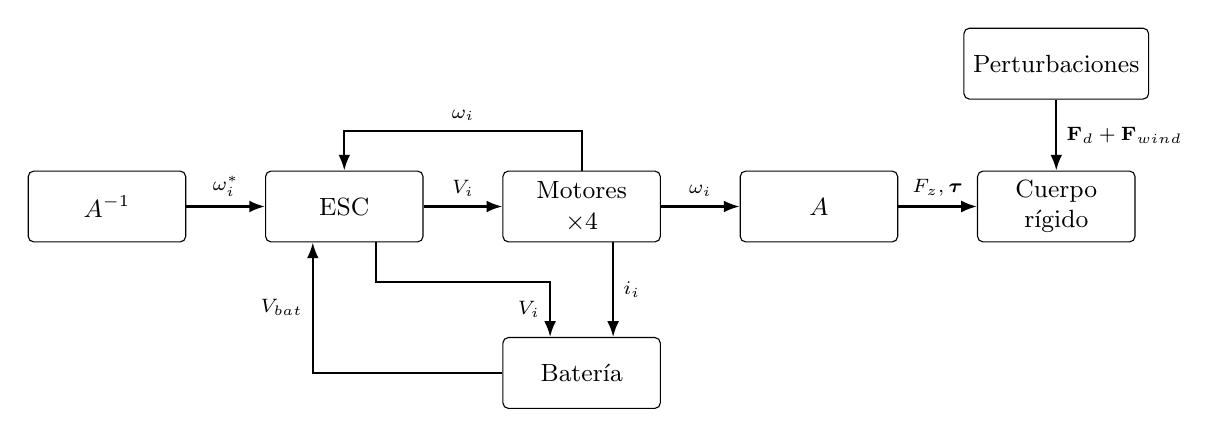
\begin{tikzpicture}[
  blk/.style={draw, rounded corners=2pt, minimum width=2.0cm, minimum height=0.9cm, align=center, font=\small},
  sig/.style={-{Latex[length=2mm]}, thick},
  node distance=0.8cm and 1.0cm]
  \node[blk] (inv) {$A^{-1}$};
  \node[blk, right=of inv] (esc) {ESC};
  \node[blk, right=of esc] (mot) {Motores\\$\times 4$};
  \node[blk, right=of mot] (A) {$A$};
  \node[blk, right=of A] (body) {Cuerpo\\rígido};
  \node[blk, below=1.2cm of mot] (bat) {Batería};
  \node[blk, above=0.9cm of body] (pert) {Perturbaciones};

  \draw[sig] (inv) -- node[above, font=\scriptsize]{$\omega_i^{*}$} (esc);
  \draw[sig] (esc) -- node[above, font=\scriptsize]{$V_i$} (mot);
  \draw[sig] (mot) -- node[above, font=\scriptsize]{$\omega_i$} (A);
  \draw[sig] (A) -- node[above, font=\scriptsize]{$F_z,\boldsymbol\tau$} (body);
  \draw[sig] (pert) -- node[right, font=\scriptsize]{$\mathbf{F}_d+\mathbf{F}_{wind}$} (body);
  \draw[sig] (mot.north) -- ++(0,0.5) -| node[pos=0.25, above, font=\scriptsize]{$\omega_i$} (esc.north);
  \draw[sig] ([xshift=4mm]mot.south) -- node[right, font=\scriptsize]{$i_i$} ([xshift=4mm]bat.north);
  \draw[sig] (bat.west) -| node[pos=0.75, left, font=\scriptsize]{$V_{bat}$} ([xshift=-4mm]esc.south);
  \draw[sig] ([xshift=4mm]esc.south) -- ++(0,-0.5) -| node[pos=0.75, left, font=\scriptsize]{$V_i$} ([xshift=-4mm]bat.north);
\end{tikzpicture}
\caption{Conexión de los subsistemas añadidos dentro de \texttt{Drone}.}
\label{fig:integracion}
\end{figure}

\subsection{Conexiones en Modelica}
\begin{lstlisting}
connect(invAllocMat.w, esc.w_ref);   // w* -> ESC
connect(esc.V, motor.V);             // V_i -> motores (vector de 4 componentes)
connect(motor.w, allocMat.w);        // w_i -> matriz de asignación
connect(motor.w, esc.w_m);           // realimentación de velocidad
connect(esc.V, bateria.V);           // potencia consumida: V_i
connect(motor.i, bateria.i);         //                   y  i_i
connect(bateria.V_bat, esc.V_bat);   // límite de tensión
connect(perturbaciones.frame_b, body.frame_a);
\end{lstlisting}

\subsection{Condiciones iniciales}
El estado inicial del cuerpo se fija explícitamente en el origen del sistema inercial,
en reposo y nivelado ($\mathbf{r}_0 = \mathbf{0}$, $\mathbf{v}_0 = \mathbf{0}$,
$\boldsymbol\eta = \mathbf{0}$, $\boldsymbol\omega = \mathbf{0}$). Son los mismos
valores que usaba implícitamente el modelo anterior. Fijarlos es necesario porque las
nuevas condiciones de régimen permanente de motores y ESC introducen ecuaciones no
lineales en la inicialización, y sin ellas el resolvedor podía desplazar la posición
inicial del cuerpo.

\subsection{Verificación}
Con los parámetros por defecto y la referencia $\mathbf{p}_{ref} = [1\;0\;1]^T$, la
trayectoria del modelo ampliado coincide con la del modelo anterior (por ejemplo,
$\mathbf{p}(\SI{2}{s}) = [0.748\;0\;0.866]^T$ frente a $[0.748\;0\;0.867]^T$), ya que
el lazo de los motores es mucho más rápido que los lazos externos. Además se han
comprobado los siguientes casos:
\begin{itemize}
  \item Carga $m_c = \SI{0.1}{kg}$ (\SI{50}{\%} de $m_d$): caída inicial de altura y
        recuperación de $z \rightarrow 1$ gracias a la acción integral.
  \item Viento $F_x = \SI{0.3}{N}$ desde $t = \SI{5}{s}$ con $c_d = \SI{0.1}{N\,s/m}$:
        desviación máxima en $x$ de unos \SI{0.46}{m} y vuelta a $x = \SI{1}{m}$.
  \item Batería de \SI{0.002}{A\,h}: la energía se agota hacia $t \approx \SI{5.5}{s}$,
        $V_{bat} \rightarrow 0$, los motores se detienen y el dron cae. La resistencia
        aerodinámica tiende a $m_{total}\,g$ (velocidad terminal).
\end{itemize}

\section{Parámetros añadidos}
\label{sec:parametros}

Los valores de la tabla~\ref{tab:parametros} son provisionales y se han elegido para
ser coherentes con $k_f$, $k_m$, $m_d$ y $\omega_{max}$ del modelo. Deben sustituirse
por los del dron comercial de referencia (Informe~1, sección~5).

\begin{table}[h]
\centering
\begin{tabular}{llll}
\toprule
Parámetro (Modelica) & Símbolo & Valor & Descripción \\
\midrule
\texttt{m\_payload}  & $m_c$      & \SI{0}{kg}              & Carga transportada \\
\texttt{R\_mot}      & $R$        & \SI{0.1}{\ohm}          & Resistencia del inducido \\
\texttt{L\_mot}      & $L$        & \SI{1e-4}{H}            & Inductancia del inducido \\
\texttt{ke}          & $k_e = k_t$ & \SI{0.005}{V\,s/rad}   & Constante contraelectromotriz / de par \\
\texttt{Jm}          & $J_m$      & \SI{2e-5}{kg\,m^2}      & Inercia motor + hélice \\
\texttt{bm}          & $b_m$      & \SI{1e-6}{N\,m\,s/rad}  & Fricción viscosa \\
\texttt{esc.kp}      & $k_p$      & \SI{0.05}{V\,s/rad}     & Ganancia proporcional del ESC \\
\texttt{esc.ki}      & $k_i$      & \SI{0.75}{V/rad}        & Ganancia integral del ESC \\
\texttt{V\_bat}      & $V_{nom}$  & \SI{7.4}{V}             & Tensión nominal (LiPo 2S) \\
\texttt{C\_bat}      & $C$        & \SI{0.5}{A\,h}          & Capacidad nominal \\
\texttt{c\_d}        & $c_d$      & \SI{0}{N\,s/m}          & Coeficiente de resistencia \\
\texttt{F\_wind}     & $\mathbf{F}_{wind}$ & $[0\;0\;0]^T$ \si{N} & Fuerza de viento (inercial) \\
\texttt{t\_wind}     & $t_{wind}$ & \SI{0}{s}               & Instante de inicio del viento \\
\texttt{w\_hover}    & $\omega_h$ & $\sqrt{m_{total} g / 4k_f}$ & Velocidad de vuelo estacionario \\
\bottomrule
\end{tabular}
\caption{Parámetros nuevos del modelo \texttt{Drone}.}
\label{tab:parametros}
\end{table}

\paragraph{Variables de interés.} Además de las variables existentes, el modelo
proporciona ahora: \texttt{motor[i].w} ($\omega_i$), \texttt{motor[i].i} ($i_i$),
\texttt{esc.V[i]} ($V_i$), \texttt{bateria.P} ($P$), \texttt{bateria.E} ($E$),
\texttt{bateria.SOC}, \texttt{perturbaciones.F} y la masa total \texttt{body.m}.
Esto cubre las magnitudes enumeradas en la sección de resultados esperados del
documento de modelado (corriente y velocidad de cada motor).

\section{Código Modelica de los subsistemas añadidos}
\label{sec:codigo}

Se muestran las ecuaciones de cada componente. Las anotaciones gráficas (iconos y
posición de los conectores) se omiten por brevedad.

\subsection{\texttt{SubSistemas.ModeloMotor}}
\begin{lstlisting}
model ModeloMotor "Equivalent DC motor + propeller load (one rotor)"
  parameter SI.Resistance R "Armature resistance";
  parameter SI.Inductance L "Armature inductance";
  parameter Real ke(unit = "V.s/rad") "Back-EMF constant";
  parameter Real kt(unit = "N.m/A") = ke "Torque constant (= ke in SI units)";
  parameter SI.Inertia Jm "Rotor inertia (motor + propeller)";
  parameter Real bm(unit = "N.m.s/rad") "Viscous friction coefficient";
  parameter Real km(unit = "N.m.s2/rad2") "Propeller torque coefficient";
  parameter Boolean steadyStateInit = true;
  parameter SI.AngularVelocity w_start = 0;

  RealInput  V(unit = "V") "Applied (equivalent) voltage";
  RealOutput w(unit = "rad/s", start = w_start) "Rotor angular speed";
  RealOutput i(unit = "A", start = km*w_start^2/kt) "Armature current";

  SI.Torque tau_m "Electromagnetic torque";
  SI.Torque tau_p "Propeller drag torque";
  SI.Power  P_el  "Electrical power drawn";
initial equation
  if steadyStateInit then
    der(i) = 0;
    der(w) = 0;
  else
    i = 0;
    w = w_start;
  end if;
equation
  L*der(i) = V - R*i - ke*w;            // modelo eléctrico
  tau_m = kt*i;
  tau_p = km*w*abs(w);                  // = km w^2 para w >= 0
  Jm*der(w) = tau_m - tau_p - bm*w;     // modelo mecánico
  P_el = V*i;
end ModeloMotor;
\end{lstlisting}

\subsection{\texttt{SubSistemas.ESC}}
\begin{lstlisting}
block ESC "Speed controller: rotor speed command -> motor voltage (4 rotors)"
  parameter SI.Resistance R;
  parameter Real ke(unit = "V.s/rad");
  parameter Real kt(unit = "N.m/A") = ke;
  parameter Real bm(unit = "N.m.s/rad");
  parameter Real km(unit = "N.m.s2/rad2");
  parameter Real kp(unit = "V.s/rad") = 0.05 "Proportional gain";
  parameter Real ki(unit = "V/rad")   = 0.75 "Integral gain";
  parameter Boolean steadyStateInit = true;

  RealInput  w_ref[4](each unit = "rad/s") "Rotor speed commands";
  RealInput  w_m[4](each unit = "rad/s")   "Measured rotor speeds";
  RealInput  V_bat(unit = "V")             "Available battery voltage";
  RealOutput V[4](each unit = "V")         "Motor voltages, 0 <= V <= V_bat";

  Real e[4], x[4](each start = 0);
  SI.Voltage V_ff[4], V_u[4];
initial equation
  if steadyStateInit then der(x) = zeros(4); else x = zeros(4); end if;
equation
  for j in 1:4 loop
    e[j]    = w_ref[j] - w_m[j];
    V_ff[j] = ke*w_ref[j] + R/kt*(km*w_ref[j]^2 + bm*w_ref[j]);
    V_u[j]  = V_ff[j] + kp*e[j] + ki*x[j];
    V[j]    = min(max(V_u[j], 0), V_bat);
    der(x[j]) = if (V_u[j] > V_bat and e[j] > 0) or (V_u[j] < 0 and e[j] < 0)
                then 0 else e[j];          // anti-windup
  end for;
end ESC;
\end{lstlisting}

\subsection{\texttt{SubSistemas.Bateria}}
\begin{lstlisting}
model Bateria "Battery as an energy reservoir with constant voltage until empty"
  parameter SI.Voltage V_nom = 7.4 "Nominal voltage";
  parameter Real C_Ah(unit = "A.h") = 0.5 "Nominal capacity";
  parameter SI.Energy E_0 = V_nom*C_Ah*3600 "Initial stored energy";

  RealInput  V[4](each unit = "V") "Motor voltages";
  RealInput  i[4](each unit = "A") "Motor currents";
  RealOutput V_bat(unit = "V")     "Available voltage";
  RealOutput SOC(unit = "1")       "State of charge E/E_0";

  SI.Energy E(start = E_0, fixed = true) "Stored energy";
  SI.Power  P "Electrical power drawn by the motors";
  Boolean empty = E <= 0;
equation
  P = sum(V[j]*i[j] for j in 1:4);
  der(E) = -P;
  V_bat = if empty then 0 else V_nom;
  SOC = E/E_0;
end Bateria;
\end{lstlisting}

\subsection{\texttt{SubSistemas.Perturbaciones}}
\begin{lstlisting}
model Perturbaciones "External forces in the inertial frame: drag + wind"
  parameter Real c_d(unit = "N.s/m") = 0 "Linear drag coefficient";
  parameter SI.Force F_wind[3] = {0, 0, 0} "Wind force, world frame";
  parameter SI.Time t_wind = 0 "Wind start time";

  Modelica.Mechanics.MultiBody.Interfaces.Frame_b frame_b;

  SI.Velocity v[3]; SI.Force F_d[3], F_w[3], F[3];
equation
  v   = der(frame_b.r_0);
  F_d = -c_d*v;
  F_w = if time >= t_wind then F_wind else zeros(3);
  F   = F_d + F_w;
  frame_b.f = -Frames.resolve2(frame_b.R, F);   // como WorldForce
  frame_b.t = zeros(3);
end Perturbaciones;
\end{lstlisting}

\subsection{Cambios en \texttt{Drone}}
\begin{lstlisting}
parameter SI.Mass m_payload = 0 "Carried payload";
parameter SI.Resistance R_mot = 0.1;  parameter SI.Inductance L_mot = 1e-4;
parameter Real ke(unit = "V.s/rad") = 0.005;
parameter SI.Inertia Jm = 2e-5;  parameter Real bm(unit = "N.m.s/rad") = 1e-6;
parameter SI.Voltage V_bat = 7.4;  parameter Real C_bat(unit = "A.h") = 0.5;
parameter Real c_d(unit = "N.s/m") = 0;
parameter SI.Force F_wind[3] = {0, 0, 0};  parameter SI.Time t_wind = 0;
parameter SI.AngularVelocity w_hover = sqrt((mass + m_payload)*g_n/(4*kf));

SubSistemas.ESC esc(R = R_mot, ke = ke, bm = bm, km = km);
SubSistemas.ModeloMotor motor[4](each R = R_mot, each L = L_mot, each ke = ke,
  each Jm = Jm, each bm = bm, each km = km, each w_start = w_hover);
SubSistemas.Bateria bateria(V_nom = V_bat, C_Ah = C_bat);
SubSistemas.Perturbaciones perturbaciones(c_d = c_d, F_wind = F_wind, t_wind = t_wind);
Modelica.Mechanics.MultiBody.Parts.Body body(m = mass + m_payload, ...,
  r_0(each fixed = true), v_0(each fixed = true),
  angles_fixed = true, w_0_fixed = true);
\end{lstlisting}


\end{document}
